\documentclass[a4paper,11pt]{article}

\usepackage[T1]{fontenc}
\usepackage[utf8]{inputenc} % bei LuaLaTeX/XeLaTeX optional
\usepackage{lmodern}

\usepackage{tikz}
\usetikzlibrary{arrows.meta,calc}

% ---- Support-Makros ----
\newcommand{\pinsupport}[1]{%
  \draw[thick] (#1) -- ++(0,-0.35);
  \draw[thick,fill=white] ($(#1)+(0,-0.35)$) ++(-0.30,0) -- ++(0.60,0) -- ++(-0.30,0.25) -- cycle;
  \draw[thick] ($(#1)+(0,-0.45)$) ++(-0.45,0) -- ++(0.90,0);
}
\newcommand{\rollersupport}[1]{%
  \draw[thick] (#1) -- ++(0,-0.35);
  \draw[thick,fill=white] ($(#1)+(0,-0.35)$) ++(-0.30,0) -- ++(0.60,0) -- ++(-0.30,0.25) -- cycle;
  \draw[thick] ($(#1)+(0,-0.42)$) ++(-0.18,0) circle (0.07);
  \draw[thick] ($(#1)+(0,-0.42)$) ++( 0.18,0) circle (0.07);
  \draw[thick] ($(#1)+(0,-0.52)$) ++(-0.45,0) -- ++(0.90,0);
}

\begin{document}

\section*{FEM-Aufgaben: Geometrie + Randbedingungen}

% ---------- Preamble (einmalig) ----------
\usepackage{tikz}
\usetikzlibrary{arrows.meta,calc}

% simple Support-Symbole (Pin / Roller)
\newcommand{\pinsupport}[1]{%
  \draw[thick] (#1) -- ++(0,-0.35);
  \draw[thick,fill=white] ($(#1)+(0,-0.35)$) ++(-0.30,0) -- ++(0.60,0) -- ++(-0.30,0.25) -- cycle;
  \draw[thick] ($(#1)+(0,-0.45)$) ++(-0.45,0) -- ++(0.90,0);
}
\newcommand{\rollersupport}[1]{%
  \draw[thick] (#1) -- ++(0,-0.35);
  \draw[thick,fill=white] ($(#1)+(0,-0.35)$) ++(-0.30,0) -- ++(0.60,0) -- ++(-0.30,0.25) -- cycle;
  \draw[thick] ($(#1)+(0,-0.42)$) ++(-0.18,0) circle (0.07);
  \draw[thick] ($(#1)+(0,-0.42)$) ++( 0.18,0) circle (0.07);
  \draw[thick] ($(#1)+(0,-0.52)$) ++(-0.45,0) -- ++(0.90,0);
}

% ---------- FIG 1: Brücke ----------
\begin{figure}[h]
\centering
\begin{minipage}{0.68\linewidth}\centering
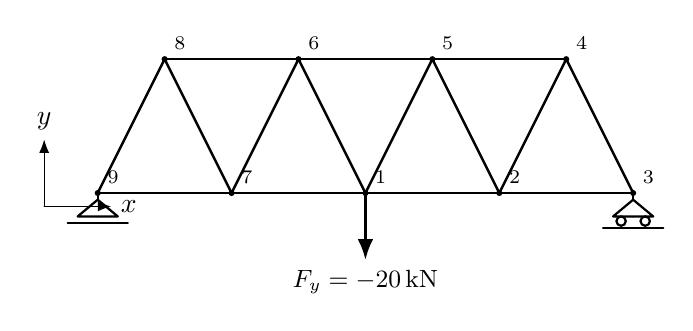
\begin{tikzpicture}[scale=0.85, line cap=round, line join=round, >=Latex]
\tikzset{truss/.style={line width=0.9pt}, load/.style={-Latex, line width=1.0pt}}

% nodes (m)
\coordinate (N1) at ( 0,0);
\coordinate (N2) at ( 2,0);
\coordinate (N3) at ( 4,0);
\coordinate (N4) at ( 3,2);
\coordinate (N5) at ( 1,2);
\coordinate (N6) at (-1,2);
\coordinate (N7) at (-2,0);
\coordinate (N8) at (-3,2);
\coordinate (N9) at (-4,0);

% elements
\draw[truss] (N9)--(N8);
\draw[truss] (N8)--(N7);
\draw[truss] (N7)--(N9);
\draw[truss] (N8)--(N6);
\draw[truss] (N6)--(N5);
\draw[truss] (N5)--(N4);
\draw[truss] (N4)--(N3);
\draw[truss] (N4)--(N2);
\draw[truss] (N2)--(N5);
\draw[truss] (N5)--(N1);
\draw[truss] (N1)--(N6);
\draw[truss] (N6)--(N7);
\draw[truss] (N7)--(N1);
\draw[truss] (N1)--(N2);
\draw[truss] (N2)--(N3);

% supports
\pinsupport{N9}      % ux=uy=0
\rollersupport{N3}   % uy=0

% load
\draw[load] (N1) -- ++(0,-1.0) node[below, font=\small] {$F_y=-20\,\mathrm{kN}$};

% node markers + ids
\foreach \i in {1,...,9}{
  \fill (N\i) circle (1.3pt);
  \node[font=\scriptsize,anchor=south west] at (N\i) {\i};
}

% axes
\draw[->] (-4.8,-0.2)--(-3.8,-0.2) node[right] {$x$};
\draw[->] (-4.8,-0.2)--(-4.8, 0.8) node[above] {$y$};
\end{tikzpicture}
\end{minipage}\hfill
\begin{minipage}{0.28\linewidth}\centering
\begin{tikzpicture}[scale=0.95, >=Latex]
\draw[->] (0,0)--(2.6,0) node[right] {$x$};
\draw[->] (0,0)--(0,1.6) node[above] {$y$};
\draw[|-|] (0,-0.45)--(2.6,-0.45) node[midway,below] {$a=8\,\mathrm{m}$};
\draw[|-|] (-0.45,0)--(-0.45,1.6) node[midway,left] {$b=2\,\mathrm{m}$};
\end{tikzpicture}
\end{minipage}

\vspace{0.6em}
\begin{tabular}{c}
\textbf{Brücke — Modellparameter}\\
$E=200\cdot10^{9}\,\mathrm{Pa}\quad;\quad A=1.6\cdot10^{-3}\,\mathrm{m^2}$\\
Last: $F_{y}(1)=-20\,\mathrm{kN}$\\
Randbedingungen: Knoten 9: $u_x=u_y=0$;\; Knoten 3: $u_y=0$
\end{tabular}
\caption{Fachwerk (Stab-FEM) — Brücke}
\end{figure}

% ---------- FIG 2: Katapult ----------
\begin{figure}[h]
\centering
\begin{minipage}{0.68\linewidth}\centering
\begin{tikzpicture}[scale=0.85, line cap=round, line join=round, >=Latex]
\tikzset{truss/.style={line width=0.9pt}, tie/.style={line width=1.1pt,dashed}, load/.style={-Latex, line width=1.0pt}}

% nodes (m)
\coordinate (N1) at (0,-1);
\coordinate (N2) at (0, 0);
\coordinate (N3) at (1, 0);
\coordinate (N4) at (0, 2);
\coordinate (N5) at (1, 2);
\coordinate (N6) at (0, 4);
\coordinate (N7) at (1, 4);
\coordinate (N8) at (0.5,6);
\coordinate (N9) at (-6,0);

% elements (1..13)
\draw[truss] (N1)--(N2);
\draw[truss] (N2)--(N3);
\draw[truss] (N3)--(N1);
\draw[truss] (N2)--(N4);
\draw[truss] (N4)--(N3);
\draw[truss] (N3)--(N5);
\draw[truss] (N5)--(N4);
\draw[truss] (N4)--(N6);
\draw[truss] (N6)--(N5);
\draw[truss] (N5)--(N7);
\draw[truss] (N7)--(N6);
\draw[truss] (N6)--(N8);
\draw[truss] (N8)--(N7);

% special element 14 (soft tie / rope)
\draw[tie] (N9)--(N2) node[midway,above, font=\scriptsize] {$E=10^{7}\,\mathrm{Pa}$};

% supports
\pinsupport{N1}
\pinsupport{N9}

% load
\draw[load] (N8) -- ++(1.1,0) node[right, font=\small] {$F_x=500\,\mathrm{N}$};

% node markers + ids
\foreach \i in {1,...,9}{
  \fill (N\i) circle (1.3pt);
  \node[font=\scriptsize,anchor=south west] at (N\i) {\i};
}

% axes
\draw[->] (-6.8,-1.2)--(-5.8,-1.2) node[right] {$x$};
\draw[->] (-6.8,-1.2)--(-6.8,-0.2) node[above] {$y$};
\end{tikzpicture}
\end{minipage}\hfill
\begin{minipage}{0.28\linewidth}\centering
\begin{tikzpicture}[scale=0.95, >=Latex]
\draw[->] (0,0)--(2.6,0) node[right] {$x$};
\draw[->] (0,0)--(0,2.6) node[above] {$y$};
\draw[|-|] (0,-0.45)--(2.6,-0.45) node[midway,below] {$a=7\,\mathrm{m}$};
\draw[|-|] (-0.45,0)--(-0.45,2.6) node[midway,left] {$b=7\,\mathrm{m}$};
\end{tikzpicture}
\end{minipage}

\vspace{0.6em}
\begin{tabular}{c}
\textbf{Katapult — Modellparameter}\\
(Hauptstäbe) $E=210\cdot10^{9}\,\mathrm{Pa}\quad;\quad A=1.0\cdot10^{-4}\,\mathrm{m^2}$\\
(Zug-/Federstab) $E=10^{7}\,\mathrm{Pa}\quad;\quad A=1.0\cdot10^{-2}\,\mathrm{m^2}$\\
Last: $F_{x}(8)=500\,\mathrm{N}$\\
Randbedingungen: Knoten 1: $u_x=u_y=0$;\; Knoten 9: $u_x=u_y=0$
\end{tabular}
\caption{Fachwerk (Stab-FEM) — Katapult}
\end{figure}

% ---------- FIG 3: Kran (E korrigiert auf 210 GPa) ----------
\begin{figure}[h]
\centering
\begin{minipage}{0.68\linewidth}\centering
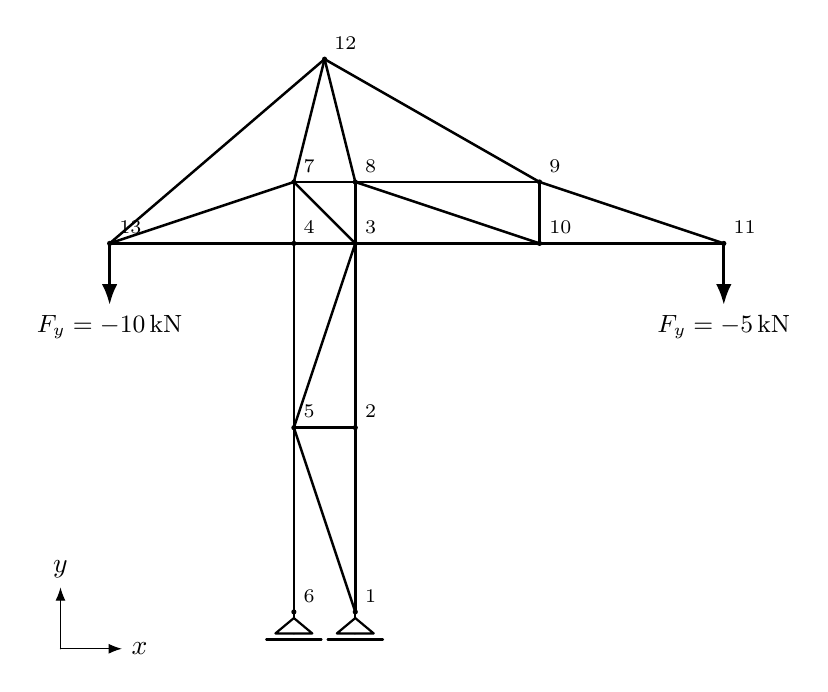
\begin{tikzpicture}[scale=0.78, line cap=round, line join=round, >=Latex]
\tikzset{truss/.style={line width=0.9pt}, load/.style={-Latex, line width=1.0pt}}

% nodes (m)
\coordinate (N1)  at (0,-6);
\coordinate (N2)  at (0,-3);
\coordinate (N3)  at (0, 0);
\coordinate (N4)  at (-1,0);
\coordinate (N5)  at (-1,-3);
\coordinate (N6)  at (-1,-6);
\coordinate (N7)  at (-1,1);
\coordinate (N8)  at (0, 1);
\coordinate (N9)  at (3, 1);
\coordinate (N10) at (3, 0);
\coordinate (N11) at (6, 0);
\coordinate (N12) at (-0.5,3);
\coordinate (N13) at (-4,0);

% elements (1..24)
\draw[truss] (N13)--(N7);
\draw[truss] (N7)--(N4);
\draw[truss] (N4)--(N13);
\draw[truss] (N13)--(N12);
\draw[truss] (N12)--(N7);
\draw[truss] (N7)--(N3);
\draw[truss] (N3)--(N4);
\draw[truss] (N4)--(N5);
\draw[truss] (N5)--(N2);
\draw[truss] (N2)--(N1);
\draw[truss] (N1)--(N5);
\draw[truss] (N5)--(N6);
\draw[truss] (N2)--(N3);
\draw[truss] (N3)--(N5);
\draw[truss] (N3)--(N8);
\draw[truss] (N8)--(N7);
\draw[truss] (N12)--(N8);
\draw[truss] (N8)--(N9);
\draw[truss] (N9)--(N12);
\draw[truss] (N3)--(N10);
\draw[truss] (N10)--(N8);
\draw[truss] (N10)--(N9);
\draw[truss] (N9)--(N11);
\draw[truss] (N11)--(N10);

% supports
\pinsupport{N1}
\pinsupport{N6}

% loads
\draw[load] (N13) -- ++(0,-1.0) node[below, font=\small] {$F_y=-10\,\mathrm{kN}$};
\draw[load] (N11) -- ++(0,-1.0) node[below, font=\small] {$F_y=-5\,\mathrm{kN}$};

% node markers + ids
\foreach \i in {1,...,13}{
  \fill (N\i) circle (1.2pt);
  \node[font=\scriptsize,anchor=south west] at (N\i) {\i};
}

% axes
\draw[->] (-4.8,-6.6)--(-3.8,-6.6) node[right] {$x$};
\draw[->] (-4.8,-6.6)--(-4.8,-5.6) node[above] {$y$};
\end{tikzpicture}
\end{minipage}\hfill
\begin{minipage}{0.28\linewidth}\centering
\begin{tikzpicture}[scale=0.95, >=Latex]
\draw[->] (0,0)--(2.6,0) node[right] {$x$};
\draw[->] (0,0)--(0,2.3) node[above] {$y$};
\draw[|-|] (0,-0.45)--(2.6,-0.45) node[midway,below] {$a=10\,\mathrm{m}$};
\draw[|-|] (-0.45,0)--(-0.45,2.3) node[midway,left] {$b=9\,\mathrm{m}$};
\end{tikzpicture}
\end{minipage}

\vspace{0.6em}
\begin{tabular}{c}
\textbf{Kran — Modellparameter}\\
\textit{(korrigiert)} $E=210\cdot10^{9}\,\mathrm{Pa}\quad;\quad A=1.0\cdot10^{-4}\,\mathrm{m^2}$\\
Lasten: $F_{y}(13)=-10\,\mathrm{kN}$;\; $F_{y}(11)=-5\,\mathrm{kN}$\\
Randbedingungen: Knoten 1: $u_x=u_y=0$;\; Knoten 6: $u_x=u_y=0$
\end{tabular}
\caption{Fachwerk (Stab-FEM) — Kran}
\end{figure}


\end{document}
